\documentclass[
aspectratio=3218, 
10pt
%, hyperref={pdfpagelabels=false}
]{beamer}

\usepackage{CJKutf8}
\usepackage[english]{babel}
%\usepackage{xcolor}
\usepackage{lmodern}
%\usepackage{amssymb}
%\usefonttheme{serif}
\usepackage[makeroom]{cancel} %for crossing symbols
\usepackage{leftindex} %For leftindex, making it possible to have nicely aligned left subscripts
%\usepackage[export]{adjustbox}
%\usepackage{calligra}
%\DeclareMathAlphabet{\mathcalligra}{T1}{calligra}{m}{n} %For small \mathcal letters
\makeatletter
\DeclareFontEncoding{LS1}{}{}
\DeclareFontSubstitution{LS1}{stix}{m}{n}
\DeclareMathAlphabet{\mathKel}{LS1}{stixscr}{m}{n}
\DeclareMathAlphabet{\mathcal}{LS1}{stixscr}{m}{n}
\usepackage{amsthm}
%\usepackage{amsmath}
%\usepackage{mathabx}
\usepackage{stmaryrd}
\usepackage{amsbsy}
\usepackage{dsfont}
\usepackage{mathtools} %für mathclap und coloneqq
%\usepackage{amsbsy}
\usepackage{mleftright} %Distanz zu \left \right weg
\usepackage{tikz-cd}

\usepackage{tabularx} %Automatic line break of tables using X instead c l r
%\usepackage{longtable} %table auf mehreren Seiten
%\usepackage{ltxtable} %Combination of both above
\usepackage{makecell} %For making larger cells in tables
\usepackage{colortbl}

\usepackage{wasysym} %Smileys!!! :)

%Für die ganzen Diagramme
\usepackage{pgfplots}

%Warning symbol
\usepackage{newunicodechar}

\newcommand\Warning{%  
\makebox[1.4em][c]{%  
\makebox[0pt][c]{\raisebox{0em}{\textbf{!}}}%  
\makebox[0pt][c]{\color{red}\LARGE$\bigtriangleup$}}}

\newunicodechar{⚠}{\Warning}

\usepackage{appendixnumberbeamer}

\usepackage{booktabs}
\usepackage[scale=2]{ccicons}

\usepgfplotslibrary{dateplot}
\usetikzlibrary{fit,
                shapes.arrows}

\usepackage{xspace}

%\usepackage{graphicx} %Für raisebox, vertical displacement of figures
\usetikzlibrary{decorations.markings, decorations.text,calc,arrows.meta}

\definecolor{Gray}{gray}{0.85}
%\usepackage[style=authortitle-icomp]{biblatex}
%\usepackage[babel,german=guillemets]{csquotes}

%\setcounter{tocdepth}{1}
%\setcounter{tocdepth}{5}
%\setcounter{secnumdepth}{4}
%\setcounter{secnumdepth}{5}
\usepackage[backend=biber, style=numeric]{biblatex}
\addbibresource{Literatur.bib}
\newcommand\fibtimes[2]{\mathbin{_{#1}\times_{#2}}}
%\newcommand{\footlineextra}[1]{
    %\begin{tikzpicture}[remember picture,overlay]
        %\node[yshift=2ex,anchor=south west] at (current page.south west) {\usebeamerfont{author in head/foot}\hspace{2ex}#1};
    %\end{tikzpicture}
%}

%\newcommand\insertreferences{}
%\setbeamertemplate{footline}{%
  %\leavevmode%
  %\hbox{%
  %\begin{beamercolorbox}[wd=.09\paperwidth, ht=5ex,dp=1ex,center, sep=1.4ex]{author in head/foot}%
    %\usebeamerfont{author in head/foot}
		%%\vfill
		%%Sources
		%%\vfill
		%Sources
  %\end{beamercolorbox}%
  %\begin{beamercolorbox}[wd=.91\paperwidth,ht=5ex,dp=1ex,center]{title in head/foot}%
    %\usebeamerfont{title in head/foot}
    %\insertreferences
%
  %\end{beamercolorbox}
%}
%}


%%% Transition slides
%\AtBeginSection[]{
  %\begin{frame}
  %%\vfill
	%\thispagestyle{empty}
  %\centering
  %\begin{beamercolorbox}[sep=8pt,center,shadow=true,rounded=true]{title}
    %\usebeamerfont{title}\insertsection\par%
  %\end{beamercolorbox}
  %%\vfill
  %\end{frame}
%}

\title{Curved Yang-Mills-Higgs theories}   
\subtitle{}   
\author{Simon-Raphael Fischer, \textit{based on joint works with Camille Laurent-Gengoux, and with Mehran Jalali Farahani, Hyungrok Kim (\begin{CJK*}{UTF8}{bkai}金炯錄\end{CJK*}), Christian Sämann}} 
\institute{
\begin{figure}
	\centering
		\includegraphics[width=.50\textwidth]{Logo_Uni_Göttingen_2022.png}
	\label{fig:NCTS}
\end{figure}
\begin{center}
%Mathematical Institute
\end{center}
}
\date{} 
%\date{Le lundi 31 mai 2021} 

% zusaetzlich ist das usepackage{beamerthemeshadow} eingebunden 
%\usepackage{beamerthemeIlmenau}
%\usepackage{beamerthemeshadow}
%\usepackage{beamerthemeDarmstadt}
%\usetheme{Arguelles}
\usetheme{metropolis}
%\usepackage[orientation=landscape,size=custom,width=16,height=9,scale=0.5,debug]{beamerposter}

%  \beamersetuncovermixins{\opaqueness<1>{25}}{\opaqueness<2->{15}}
%  sorgt dafuer das die Elemente die erst noch (zukuenftig) kommen 
%  nur schwach angedeutet erscheinen 
\beamersetuncovermixins{\opaqueness<1>{25}}{\opaqueness<2->{15}}
% klappt auch bei Tabellen, wenn teTeX verwendent wird\ldots

\beamertemplatenavigationsymbolsempty %Damit sind die kleinen Navigationssymbole unten weg

%\usesectionheadtemplate{}{}
%\usesubsectionheadtemplate{}{}

\def\be{\begin{equation}}
\def\ee{\end{equation}}
\def\bs{\begin{subequations}}
\def\es{\end{subequations}}
\def\ba#1\ea{\begin{align}#1\end{align}}
\def\bes{\begin{equation*}}
\def\ees{\end{equation*}}
\def\bas#1\eas{\begin{align*}#1\end{align*}}

\AtBeginEnvironment{remark}{%
  \setbeamercolor{block title}{use=example text,fg=black,bg=yellow!75!black}
  \setbeamercolor{block body}{parent=normal text,use=block title example,bg=yellow!10}
}
\AtBeginEnvironment{motivation}{%
  \setbeamercolor{block title}{use=example text,fg=black,bg=yellow!75!black}
  \setbeamercolor{block body}{parent=normal text,use=block title example,bg=yellow!10}
}
%\AtBeginEnvironment{example}{%
  %\setbeamercolor{block title}{use=example text,fg=black,bg=green!75!black}
  %\setbeamercolor{block body}{parent=normal text,use=block title example,bg=green!10}
%}

\renewcommand{\qedsymbol}{}
\theoremstyle{plain}
\newtheorem{conjecture}[theorem]{Conjecture}
\newtheorem{proposition}[theorem]{Proposition}
%\newtheorem{definition}[theorem]{Definition}
\theoremstyle{remark}
\newtheorem*{remark}{Remarks}
\newtheorem*{gedankenexperiment}{Gedankenexperiment}
\newtheorem*{idea}{Idea}
\newtheorem*{motivation}{Motivation}
\newtheorem*{summary}{Summary}
\newtheorem*{situation}{Situation}
\newtheorem*{lab}{Situation: Lie algebra bundles}
\newtheorem*{question}{Question}
\newtheorem*{fieldredefinition}{Field Redefinition}
\newtheorem*{construction}{Construction}
\newtheorem*{aim}{Aim}
\newtheorem*{BackToTheRoots}{Back to the roots}

\AtBeginEnvironment{BackToTheRoots}{%
  \setbeamercolor{block title}{use=example text,fg=black,bg=pink!75!black}
  \setbeamercolor{block body}{parent=normal text,use=block title example,bg=pink!10}
}
\AtBeginEnvironment{gedankenexperiment}{%
  \setbeamercolor{block title}{use=example text,fg=black,bg=pink!75!black}
  \setbeamercolor{block body}{parent=normal text,use=block title example,bg=pink!10}
}
\AtBeginEnvironment{idea}{%
  \setbeamercolor{block title}{use=example text,fg=black,bg=pink!75!black}
  \setbeamercolor{block body}{parent=normal text,use=block title example,bg=pink!10}
}

%\theoremstyle{definition}
%\newtheorem{definition}[theorem]{Definition}
%\newtheorem*{SecondIn}{Second Inequality}

%mathrm mit mathup ersetzen, damit die font passt
\renewcommand\familydefault{\sfdefault} %comment to see the difference
\DeclareMathAlphabet      {\mathup}{OT1}{\familydefault}{m}{n}


\begin{document}


\begin{frame}
\thispagestyle{empty}
\titlepage
\end{frame} 


{
\setbeamertemplate{footline}{}
\begin{frame}
%\frametitle{Table of contents}
%\tableofcontents
\thispagestyle{empty}
\begin{figure}[htbp]
	\centering
		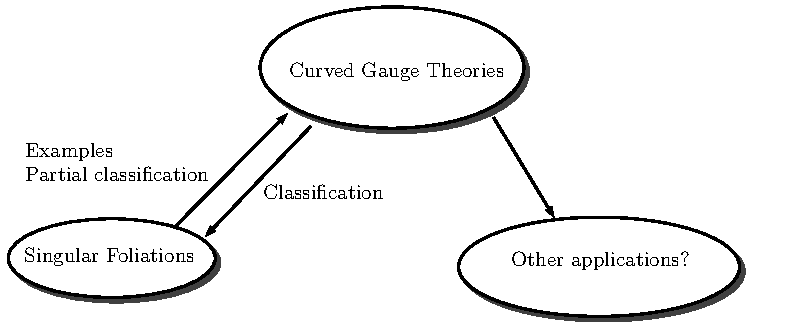
\includegraphics[width=1\textwidth]{Research circles I.pdf}
\end{figure}
\end{frame} 
}

\section{Motivation}



\begin{frame}{Motivation: Covariantisation of Yang-Mills(-Higgs) theory}
\begin{tikzpicture}
\coordinate (a) at (0, 0);
\coordinate (b) at (15, 0);
\path[->, line width=1mm] (a) edge node[above] {Covariantization} (b);
\end{tikzpicture}
{\renewcommand{\arraystretch}{2}
\begin{table}[h!]
		\begin{tabularx}{\textwidth}{c c c}
			\rowcolor{gray}
			Classical theory & Covariantised flat theory & Curved Theory \\
			Vector space $V$ & Trivial vector bundle $M \times V$ & Vector bundle $V \to M$ \\
			\rowcolor{Gray}
			$\frac{\partial}{\partial x^i}$ & Canonical flat connection $\nabla^0$ & Vector bundle connection $\nabla$ \\ 
			\multicolumn{1}{X}{Coordinate changes may lead to extra terms} & 
			\multicolumn{2}{c}{Coordinate expressions form-invariant under coordinate changes}
		\end{tabularx}
\end{table}}
\vspace{-30pt}
\begin{tikzcd}[ampersand replacement=\&]
\phantom{Coordinate changes may lead to extra terms} \arrow[bend right, equal]{r} \& \phantom{Coordinate}
	\end{tikzcd}
 \end{frame}

\setbeamertemplate{frame footer}{S.-R.\ Fischer. \textit{Integrating curved Yang–Mills gauge theories}, arXiv: 2210.02924, 2022. \newline 
S.-R.\ Fischer. \textit{Geometry of curved Yang–Mills–Higgs gauge theories}, Ph.D.\ thesis, Institut Camille Jordan [Villeurbanne], France, U. Geneva, Switzerland, 2021; doi: 10.13097/archive-ouverte/unige:152555}

\begin{frame}{Curved Yang-Mills gauge theory (curved YM theory)}
\begin{tikzpicture}
\coordinate (a) at (0, 0);
\coordinate (b) at (15, 0);
\path[->, line width=1mm] (a) edge node[above] {Covariantization} (b);
\end{tikzpicture}
{\renewcommand{\arraystretch}{2}
\begin{table}[h!]
		\begin{tabularx}{\textwidth}{c c c}
			\rowcolor{gray}
			YM theory & Covariantised YM theory & Curved YM theory \\
			Lie group $G$ & Trivial Lie group bundle $M \times G$ & Lie group bundle $G \to M$ \\
			\rowcolor{Gray}
			Maurer-Cartan form & Fibre-wise Maurer-Cartan & Multiplicative YM connection \\ 
			\multicolumn{1}{X}{Field redefinitions lead to extra terms in gauge transformations and field strength} & 
			\multicolumn{2}{c}{\makecell{Expressions form-invariant under field redefinitions, \\ \textbf{but curvature transforms non-trivially}}}
		\end{tabularx}
\end{table}}
\vspace{-30pt}
\begin{tikzcd}[ampersand replacement=\&]
\phantom{Coordinate changes may lead to extra terms} \arrow[bend right, equal]{r} \& \phantom{Coordinate}
	\end{tikzcd}
\end{frame}

\setbeamertemplate{frame footer}{S.-R.\ Fischer, M.\ Jalali Farahani, H.\ Kim, and C.\ Saemann. \textit{Adjusted connections I: Differential cocycles for principal groupoid bundles with connection}, arXiv: 2406.16755, 202. \newline 
S.-R.\ Fischer. \textit{Geometry of curved Yang–Mills–Higgs gauge theories}, Ph.D.\ thesis, Institut Camille Jordan [Villeurbanne], France, U. Geneva, Switzerland, 2021; doi: 10.13097/archive-ouverte/unige:152555}

\begin{frame}{Curved Yang-Mills-Higgs theory (curved YMH theory)}
\begin{tikzpicture}
\coordinate (a) at (0, 0);
\coordinate (b) at (15, 0);
\path[->, line width=1mm] (a) edge node[above] {Covariantization} (b);
\end{tikzpicture}
{\renewcommand{\arraystretch}{2}
\begin{table}[h!]
		\begin{tabularx}{\textwidth}{c c c}
			\rowcolor{gray}
			YMH theory & Covariantised YMH theory & Curved YMH theory \\
			Lie group $G$ with right-action on $N$ & Action groupoid $N \times G$ & Lie groupoid $G \rightrightarrows N$ \\
			\rowcolor{Gray}
			Maurer-Cartan form & Fibre-wise Maurer-Cartan & Covariant adjustments \\ 
			\multicolumn{1}{X}{Field redefinitions lead to extra terms in gauge transformations and field strength} & 
			\multicolumn{2}{c}{\makecell{Expressions form-invariant under field redefinitions, \\ \textbf{but curvature transforms non-trivially}}}
		\end{tabularx}
\end{table}}
\vspace{-30pt}
\begin{tikzcd}[ampersand replacement=\&]
\phantom{Coordinate changes may lead to extra terms} \arrow[bend right, equal]{r} \& \phantom{Expressions form-invariant}
	\end{tikzcd}
\end{frame}

\section{Lie groupoids}

{
\setbeamertemplate{frame footer}{Ana Cannas Da Silva and Alan Weinstein. \textit{Geometric models for noncommutative algebras}, volume 10. American Mathematical Soc., 1999.}

\begin{frame}
\begin{center}
	\begin{tikzcd}[ampersand replacement=\&]
x'' \& \arrow[l, swap, "g'", bend right] x' \& \arrow[l, swap, "g", bend right] \arrow[ll, swap, "g'g", bend right=70] x
	\end{tikzcd}
\end{center}
\end{frame}


\begin{frame}
\begin{center}
	\begin{tikzcd}[ampersand replacement=\&]
\mathcal{G} \arrow[d, shift left, "s"]\arrow["t", swap, shift right]{d} \\
	N
	\end{tikzcd}
\end{center}

\begin{definition}[Lie groupoids]
\vspace{.5pt}
$\mathcal{G}$ a \textbf{Lie groupoid} if there are surjective submersions $s, t \colon \mathcal{G} \to N$,  \textit{source} and \textit{target}, respectively, and a smooth \textit{multiplication map} $\mathcal{G} \fibtimes{s}{t} \mathcal{G} \to \mathcal{G}$ such that 
\bes
s(g'g) = s(g), \qquad t(g'g) = t(g')
\ees
for all $(g', g) \in \mathcal{G} \fibtimes{s}{t} \mathcal{G}$ (i.e.\ $s(g') = t(g)$), satisfying the typical expected properties, that is,
\bas
\text{Associativity:} && (g'' g') g &= g'' (g'g),
\\
\text{Units:} && g e_{s(g)} = g, \quad&\quad e_{t(g)} g = g,
\\
\text{Inverse:} && g^{-1} g = e_{s(g)}, \quad&\quad g g^{-1} = e_{t(g)}
\eas
for all $(g'', g', g) \in \mathcal{G} \fibtimes{s}{t} \mathcal{G} \fibtimes{s}{t} \mathcal{G}$, where one requires the existence of the \textit{unit} $e$ as a global section of both, $s$ and $t$, and the \textit{inverse} $g^{-1} \in \mathcal{G}$ of $g$.
\end{definition}
\end{frame}

\begin{frame}
\begin{center}
	\begin{tikzcd}[ampersand replacement=\&]
* \& \arrow[l, swap, "g'", bend right] * \& \arrow[l, swap, "g", bend right] \arrow[ll, swap, "g'g", bend right=70] *
	\end{tikzcd}
\end{center}
%\pause
\begin{example}[Lie groups]
\vspace{.5pt}
Lie groups $G$
\begin{center}
	\begin{tikzcd}[ampersand replacement=\&]
G \arrow[d, shift left, "s"]\arrow["t", swap, shift right]{d} \\
	\{*\}
	\end{tikzcd}
\end{center}
\end{example}
\end{frame}

\begin{frame}
\begin{center}
	\begin{tikzcd}[ampersand replacement=\&]
x \& \arrow[l, swap, "g'", bend right] x \& \arrow[l, swap, "g", bend right] \arrow[ll, swap, "g'g", bend right=70] x
	\end{tikzcd}
\end{center}

\begin{example}[Lie group bundles (LGBs)]
\vspace{.5pt}
LGB $\pi_G \colon G \to M$
\begin{center}
	\begin{tikzcd}[ampersand replacement=\&]
G \arrow[d, shift left, "\pi_G"]\arrow["\pi_G", swap, shift right]{d} \\
	M
	\end{tikzcd}
\end{center}
\end{example}
\end{frame}


\begin{frame}
\begin{center}
	\begin{tikzcd}[ampersand replacement=\&]
x \& \arrow[l, swap, "g'" pos=.42, bend right] x \cdot q \& \arrow[l, swap, "g" pos= .45, bend right] \arrow[ll, swap, "g'g", bend right=70] x \cdot q q'
	\end{tikzcd}
\end{center}


\begin{example}[Action groupoid (trivial)]
\vspace{.5pt}
Lie group $G$ with action $\Psi \colon N \times G \to N$, $(p, q) \mapsto p \cdot q$, on $N$. 
\begin{center}
	\begin{tikzcd}[ampersand replacement=\&]
N \times G \arrow[d, shift left, "\Psi"]\arrow["\mathup{pr}_1", swap, shift right]{d} \\
	N
	\end{tikzcd}
\bas
(x, q) ~ (x \cdot q, q')&=(x, q q')~,
\\
e_x &= \left(x, e \right)~,
\\
(x, q)^{-1} &= \left(x \cdot q, q^{-1} \right)
\eas
\end{center}
\end{example}
\end{frame}

\setbeamertemplate{frame footer}{Kirill C.~H.\ Mackenzie. \textit{General theory of {L}ie groupoids and {L}ie algebroids}, London Mathematical Society Lecture Note Series, 213:xxxviii+501, 2005.}

\begin{frame}
\begin{center}
	\begin{tikzcd}[ampersand replacement=\&]
P \arrow["\Phi", swap]{rd} \& \arrow[bend right]{l} \mathcal{G} \arrow[d, shift left, "s"]\arrow["t", swap, shift right]{d} \\
	 \& N
	\end{tikzcd}
\end{center}

\begin{definition}[Groupoid right-action]\vspace{.5pt}
A \textbf{right-action} is a smooth map $P \fibtimes{\Phi}t \mathcal{G} \to P$ such that
\bas
\Phi(p \cdot g') &= s(g'),
\\
(p \cdot g') \cdot g &= p \cdot (g' g),
\\
p \cdot e_{\Phi(p)} &= p
\eas
for all $(p, g', g) \in P \fibtimes{\Phi}t \mathcal{G} \fibtimes ts \mathcal{G}$.
\end{definition}
\end{frame}

\section{Principal bundles and their Ehresmann connections}

\setbeamertemplate{frame footer}{I.~Moerdijk and J.~Mr{\v c}un. \textit{Introduction to foliations and Lie groupoids}, Cambridge University Press, 2003.}

\begin{frame}
\begin{center}
	\begin{tikzcd}[ampersand replacement=\&]
P \arrow["\Phi", swap]{rd} \arrow["\pi", swap]{d} \& \arrow[bend right]{l} \mathcal{G} \arrow[d, shift left, "s"]\arrow["t", swap, shift right]{d} \\
	M \& N
	\end{tikzcd}
\end{center}

\begin{definition}[Principal groupoid-bundles]\vspace{.5pt}
$\pi\colon P \to M$ surjective submersion is a \textbf{principal $\mathcal{G}$-bundle} if
\bes
\pi(p \cdot g) = \pi(p)
\ees
for all $(p, g) \in P \fibtimes{\Phi}t \mathcal{G}$,
and if
\bas
P \fibtimes{\Phi}t \mathcal{G} &\to P \fibtimes\pi\pi P,
\\
(p, g) &\mapsto (p, p\cdot g)
\eas
is a diffeomorphism.
\end{definition}
\end{frame}

\setbeamertemplate{frame footer}{}

\begin{frame}{Ehresmann connection}
\begin{center}
	\begin{tikzcd}[ampersand replacement=\&]
P \arrow["\Phi", swap]{rd} \arrow["\pi", swap]{d} \& \arrow[bend right]{l} \mathcal{G} \arrow[d, shift left, "s"]\arrow["t", swap, shift right]{d} \\
	M \& N
	\end{tikzcd}
\end{center}

\begin{remark}
Infinitesimal action:
\bas
\mathup{T}P \fibtimes{\mathup{D}\Phi}{\mathup{D}t} \mathup{T}\mathcal{G}
&\to 
\mathup{T}P,
\\
(X, Y) &\mapsto X \cdot Y.
\eas
\pause
For $r_g(p) \coloneqq p \cdot g$ with $\Phi(p) = t(g)$, its infinitesimal version corresponds to
\bes
\mathup{D}r_g(X) = X \cdot 0
\ees
for all $X$ with $\mathup{D}\Phi(X) = 0$.
\end{remark}
\end{frame}

\setbeamertemplate{frame footer}{I.~Moerdijk and J.~Mr{\v c}un. \textit{Introduction to foliations and Lie groupoids}, Cambridge University Press, 2003. \newline
D.~Signori and M.~Sti\'{e}non. \textit{On nonlinear gauge theories}, J.\ Geom.\ Phys.\ {\bf 59} 1063, 2009.}

\begin{frame}{Ehresmann connection}
\begin{center}
	\begin{tikzcd}[ampersand replacement=\&]
P \arrow["\Phi", swap]{rd} \arrow["\pi", swap]{d} \& \arrow[bend right]{l} \mathcal{G} \arrow[d, shift left, "s"]\arrow["t", swap, shift right]{d} \\
	M \& N
	\end{tikzcd}
\end{center}

Infinitesimal $\mathcal{G}$-action on $P$:
\bas
\mathup{T}P \fibtimes{\mathup{D}\Phi}{\mathup{D}t} \mathup{T}\mathcal{G}
&\to 
\mathup{T}P,
\\
(X, Y) &\mapsto X \cdot Y.
\eas

\begin{idea}
Horizontal distribution $\mathup{H}P$ (w.r.t.\ $\pi$) with
\bes
\mathup{D}\Phi ( \mathup{H}P ) = 0.
\ees
\end{idea}

\end{frame}

\setbeamertemplate{frame footer}{S.-R.\ Fischer. \textit{Integrating curved Yang–Mills gauge theories}, arXiv: 2210.02924, 2022. \newline 
S.-R.\ Fischer. \textit{Geometry of curved Yang–Mills–Higgs gauge theories}, Ph.D.\ thesis, Institut Camille Jordan [Villeurbanne], France, U. Geneva, Switzerland, 2021; doi: 10.13097/archive-ouverte/unige:152555}


\begin{frame}{We lose covariantization}


%\begin{center}
{\renewcommand{\arraystretch}{2}
\begin{table}[h!]
\centering
		\begin{tabularx}{\textwidth}{c c c}
			%\rowcolor{gray}
			 & \cellcolor{gray} YM theory & \cellcolor{gray} Covariantised YM theory\\
			\phantom{assssssssdasdasdasd} & Lie group $G$ & Trivial Lie group bundle $M \times G$ \\
			%\rowcolor{Gray}
			 & \cellcolor{Gray} Maurer-Cartan form & \cellcolor{Gray} Fibre-wise Maurer-Cartan
		\end{tabularx}
\end{table}}

\begin{center}
\vspace{-25pt}
\begin{tikzcd}[ampersand replacement=\&]
\phantom{Maurer-Cartan form} \arrow[bend right, equal]{r} \& \phantom{Fibre-wise Maurer-Cartan}
	\end{tikzcd}
\end{center}
%\end{center}
	
	
\begin{center}
\Warning We would lose the equivalence to the covariantised theory where we set $\Phi = \pi$ \Warning
\end{center}

\begin{center}
	\begin{tikzcd}[ampersand replacement=\&]
P \arrow["\Phi"]{rd} \arrow["\pi", swap]{d} \& \arrow[bend right]{l} M \times G \arrow{d} \\
	M \arrow[equal]{r} \& M
	\end{tikzcd}
\end{center}
\end{frame}

\setbeamertemplate{frame footer}{
S.-R.\ Fischer, M.\ Jalali Farahani, H.\ Kim, and C.\ Saemann. \textit{Adjusted connections I: Differential cocycles for principal groupoid bundles with connection}, arXiv: 2406.16755, 202. \newline 
S.-R.\ Fischer. \textit{Integrating curved Yang–Mills gauge theories}, arXiv: 2210.02924, 2022.}

\begin{frame}{New idea!}
\begin{center}
	\begin{tikzcd}[ampersand replacement=\&]
P \arrow["\Phi", swap]{rd} \arrow["\pi", swap]{d} \& \arrow[bend right]{l} \mathcal{G} \arrow[d, shift left, "s"]\arrow["t", swap, shift right]{d} \\
	M \& N
	\end{tikzcd}
\end{center}

\begin{idea}[Ehresmann connection on $P$]
Equip $\mathcal{G}$ with a horizontal distribution $\mathup{H}\mathcal{G}$ (w.r.t.\ $t$). An Ehresmann connection on $P$ is a horizontal distribution $\mathup{H}P$ (w.r.t.\ $\pi$) so that the infinitesimal $\mathcal{G}$-action on $P$ restricts 
\bes
\mathup{H}P \fibtimes{\mathup{D}\Phi}{\mathup{D}t} \mathup{H}\mathcal{G}
\to 
\mathup{H}P.
\ees
\pause
Invariance then via the \textbf{modified right-pushforward $\mathcal{r}_{g*}$}
\bes
\mathcal{r}_{g*}(X) \coloneqq X \cdot Y
\ees
for all $X \in \mathup{T}_pP$, where $Y \in \mathup{H}_g\mathcal{G}$ is the unique lift of $\mathup{D}_p\Phi(X)$.
\end{idea}

\end{frame}

\begin{frame}
\begin{idea}
$\mathup{H}P$ Ehresmann, then
\bes
\mathup{H}P \fibtimes{\mathup{D}\Phi}{\mathup{D}t} \mathup{H}\mathcal{G}
\to 
\mathup{H}P.
\ees
\end{idea}

\begin{theorem}\vspace{.5pt}
Given such an $\mathup{H}P$, then $\mathup{H}\mathcal{G}$ is \textbf{Cartan},
\bes
\mathup{H}\mathcal{G} \fibtimes{\mathup{D}s}{\mathup{D}t} \mathup{H}\mathcal{G}
\to 
\mathup{H}\mathcal{G}.
\ees
\end{theorem}
\pause
\begin{proof}[Sketch as a proof for LGBs]\vspace{.5pt}
W.r.t.\ parallel transports we have
\bes
\mathup{PT}^P(p\cdot g) = \mathup{PT}^P(p) \cdot \mathup{PT}^{\mathcal{G}}(g).
\ees
\end{proof}
\end{frame}

\begin{frame}
\begin{theorem}\vspace{.5pt}
Given such an $\mathup{H}P$, then $\mathup{H}\mathcal{G}$ is \textbf{Cartan},
\bes
\mathup{H}\mathcal{G} \fibtimes{\mathup{D}s}{\mathup{D}t} \mathup{H}\mathcal{G}
\to 
\mathup{H}\mathcal{G}.
\ees
\end{theorem}

\begin{proof}[Sketch as a proof for LGBs]\vspace{.5pt}
W.r.t.\ parallel transports we have
\bes
\mathup{PT}^P(p\cdot g) = \mathup{PT}^P(p) \cdot \mathup{PT}^{\mathcal{G}}(g),
\ees
then
\begin{center}
\begin{tikzcd}[ampersand replacement=\&]
\mathup{PT}^P\bigl(p\cdot (gq)\bigr) \arrow[equal]{d} 
\& \arrow[equal]{l} \mathup{PT}^P(p) \cdot \mathup{PT}^{\mathcal{G}}(gq)
\\
\mathup{PT}^P\bigl((p\cdot g) \cdot q\bigr) \arrow[equal]{r}
\& \mathup{PT}^P(p) \cdot \mleft( \mathup{PT}^{\mathcal{G}}(g) ~ \mathup{PT}^{\mathcal{G}}(q) \mright).
\end{tikzcd}
\end{center}
\end{proof}
\end{frame}

\begin{frame}
\begin{idea}
$\mathup{H}P$ Ehresmann, then
\bes
\mathup{H}P \fibtimes{\mathup{D}\Phi}{\mathup{D}t} \mathup{H}\mathcal{G}
\to 
\mathup{H}P.
\ees
\end{idea}

\begin{theorem}\vspace{.5pt}
Given such an $\mathup{H}P$, then $\mathup{H}\mathcal{G}$ is \textbf{Cartan},
\bes
\mathup{H}\mathcal{G} \fibtimes{\mathup{D}s}{\mathup{D}t} \mathup{H}\mathcal{G}
\to 
\mathup{H}\mathcal{G}.
\ees
\end{theorem}

\begin{remark}
Vice versa, if $\mathup{H}\mathcal{G}$ is Cartan, then such $\mathup{H}P$ exist.
\end{remark}
\end{frame}

\setbeamertemplate{frame footer}{}

\begin{frame}{What else?}
\begin{idea}
Open a textbook about ordinary gauge theory, and replace:
\begin{itemize}
	\item Right-pushforward $\rightsquigarrow$ Modified right-pushforward,
	\item Adjoint representation $\rightsquigarrow$ Adjoint representation via Cartan connections (?)
	\item Generalising the concept of field strength accounting for a possible curvature coming from $\mathcal{G}$
\end{itemize}
Too much to introduce! (Lie algebroids, Lie algebroid connections, basic curvature, basic connections, and so on...)

Thus, for today: LGBs!
\end{idea}
\end{frame}

\section{Curved Yang-Mills gauge theory}

\setbeamertemplate{frame footer}{
S.-R.\ Fischer. \textit{Integrating curved Yang–Mills gauge theories}, arXiv: 2210.02924, 2022.}

\begin{frame}
\begin{remark}
The groupoid is now an LGB $\pi_{\mathcal{G}} \colon \mathcal{G} \to M$ with structural Lie group $G$.
\end{remark}

%\begin{remark}
Gauge invariance requires us to study \emph{special} Cartan connections:
%\end{remark}

\begin{definition}[Multiplicative Yang-Mills connections]\vspace{.5pt}
A connection 1-form $\mu_{\mathcal{G}}$ on the LGB $\mathcal{G}$ is a \textbf{multiplicative Yang-Mills connection (w.r.t.\ a $\zeta \in \Omega^2(M; \mathcal{g})$)} if it is a Cartan connection satisfying the \textbf{generalised Maurer-Cartan equation}:
	\bas
	\mleft.\mleft(\mathrm{d}^{\pi_{\mathcal{G}}^*\nabla^{\mathcal{G}}} \mu_{\mathcal{G}}
	+ \frac{1}{2} \mleft[ \mu_{\mathcal{G}} \stackrel{\wedge}{,} \mu_{\mathcal{G}} \mright]_{\pi_{\mathcal{G}}^*\mathcal{g}} \mright)\mright|_g
&=
\mathrm{Ad}_{g^{-1}} \circ \mleft.\pi_{\mathcal{G}}^!\zeta\mright|_g
	- \mleft.\pi_{\mathcal{G}}^!\zeta\mright|_g
	\eas
for all $g \in \mathcal{G}$, where $\mathcal{g}$ is the Lie algebra bundle (LAB) of $\mathcal{G}$, and $\nabla^\mathcal{G}$ is the naturally induced LAB connection.
\end{definition}

\pause

\begin{remark}[Closed connection, exact curvature]
\bes
R_{\nabla^{\mathcal{G}}} = \mathup{ad} \circ \zeta.
\ees
\end{remark}
\end{frame}

\begin{frame}
\begin{definition}\vspace{.5pt}
The field strength $F$ of an Ehresmann connection $A \in \Omega^1(P; \pi^*\mathcal{g})$ on $\pi \colon P \to M$ is defined by 
\bes
F
\coloneqq
\mathrm{d}^{\pi^*\nabla^{\mathcal{G}}} A
	+ \frac{1}{2} \mleft[ A \stackrel{\wedge}{,} A \mright]_{\pi^*\mathcal{g}}
	+ \pi^!\zeta.
\ees
\end{definition}
\pause
\begin{theorem}\vspace{.5pt}
By contracting $F$ with an $\mathup{ad}$-invariant scalar product we achieve a gauge-invariant Lagrangian $\mathcal{L}[A]$, that is,
\bes
\mathcal{L}\mleft[L^!A\mright]
=
\mathcal{L}[A]
\ees
for all $L \in \mathup{Aut}(P)$.
\end{theorem}
\end{frame}

\section{Examples}

\setbeamertemplate{frame footer}{
Kirill C.~H.\ Mackenzie. \textit{General theory of {L}ie groupoids and {L}ie algebroids}, London Mathematical Society Lecture Note Series, 213:xxxviii+501, 2005.\newline
S.-R.\ Fischer. \textit{Curved {Y}ang–{M}ills–{H}iggs gauge theories in the case of
  massless gauge bosons}, Journal of Geometry and Physics, 162:104104, 2021.
}

\begin{frame}
\begin{idea}
Let us assume that the structural Lie group $G$ is semisimple, then:
\end{idea}

\begin{theorem}\vspace{.5pt}
There is a unique (up to isomorphism) principal $G$-bundle $Q$ such that 
\bes
\mathcal{G} = (Q\times G) \Big/ G,
\ees
multiplicative Yang-Mills connections on $\mathcal{G}$ are precisely associated connections, thus in 1:1 correspondence to Ehresmann connections on $Q$, and $\zeta$ is the corresponding curvature on $Q$.
\end{theorem}
\end{frame}

\setbeamertemplate{frame footer}{
S.-R.\ Fischer. \textit{Curved {Y}ang–{M}ills–{H}iggs gauge theories in the case of
  massless gauge bosons}, Journal of Geometry and Physics, 162:104104, 2021.
}

\begin{frame}
\begin{corollary}\vspace{.5pt}
There are only curved multiplicative Yang-Mills connections on $\mathcal{G}$ if and only if $Q$ is not flat.
\end{corollary}

\begin{example}\vspace{.5pt}
Hopf fibration $Q \coloneqq \mathbb{S}^7 \to \mathbb{S}^4$,
\bes
\mathcal{G} = \bigl( Q \times \mathup{SU}(2) \bigr) \Big/ \mathup{SU}(2).
\ees
\end{example}

\pause

\begin{remark}
Some technical details:
\begin{itemize}
	\item This is stable under field redefinitions.
	\item This can be relaxed to $\mathcal{G}$ with a trivial centre, using a nice geometric interpretation via singular foliations. However, dynamics of gauge theory require $\mathup{Ad}$-invariance...
	
	See Camille's talk on Friday \smiley
\end{itemize}
\end{remark}
\end{frame}

\setbeamertemplate{frame footer}{
S.-R.\ Fischer, M.\ Jalali Farahani, H.\ Kim, and C.\ Saemann. \textit{Adjusted connections I: Differential cocycles for principal groupoid bundles with connection}, arXiv: 2406.16755, 202.}

\begin{frame}{About Lie groupoids...}
\begin{idea}
Assume that $G$ is semisimple \textbf{and} acts faithfully on $\mathbb{R}^d$ fixing $0$. Then $\mathcal{G}$ acts faithfully on 
\bes
N
\coloneqq 
\mleft(Q \times \mathbb{R}^d\mright) \Big/ G,
\ees
giving rise to an action groupoid structure on $\phi^*\mathcal{G}$ ($\phi \colon N \to M$)
\begin{center}
	\begin{tikzcd}[ampersand replacement=\&]
\phi^*\mathcal{G} \arrow[d, shift left, "s"]\arrow["t", swap, shift right]{d} \\
	N
	\end{tikzcd}
\end{center}
\end{idea}
\pause
\begin{theorem}\vspace{.5pt}
The pullback of the multiplicative Yang-Mills connection on $\phi^*\mathcal{G}$ is flat up to field redefinitions if and only if $Q$ is flat.
\end{theorem}
\end{frame}

\begin{frame}
\begin{theorem}\vspace{.5pt}
The pullback of the multiplicative Yang-Mills connection on $\phi^*\mathcal{G}$ is flat up to field redefinitions if and only if $Q$ is flat.
\end{theorem}

\begin{remark}
Other technical details:
\begin{itemize}
	\item Also stable under field redefinitions!
	\item Here semi-simplicity is rather important.
\end{itemize}
\end{remark}
\pause
\begin{example}\vspace{.5pt}
Again $Q$ the Hopf fibration $\mathbb{S}^7 \to \mathbb{S}^4$, then naturally choose $\mathbb{R}^d = \mathbb{C}^2$.
\end{example}
\end{frame}


\begin{frame}{Outlook}
\end{frame}


\begin{frame}[standout]
\thispagestyle{empty}
\topmargin -3.46 cm
\vspace*{\fill}
\begin{center}
\huge \textbf{Thank you!}
\end{center}
\vspace*{\fill}
\end{frame}

\appendix

\setbeamertemplate{frame footer}{
S.-R.\ Fischer. \textit{Geometry of curved Yang–Mills–Higgs gauge theories}, Ph.D.\ thesis, Institut Camille Jordan [Villeurbanne], France, U. Geneva, Switzerland, 2021; doi: 10.13097/archive-ouverte/unige:152555
}

\begin{frame}[fragile]{A quick funny example, again by $\mathbb{S}^7$}
\begin{example}\vspace{.5pt}
The Lie groupoid $\mathcal{G}$ given as the pair groupoid of $\mathbb{S}^7$ leads to descriptions of curved Yang-Mills-Higgs theories, which cannot be described in an ordinary way due to the lack of non-associativity on $\mathbb{S}^7$.
\end{example}
\end{frame}

\end{document}

